% Options for packages loaded elsewhere
\PassOptionsToPackage{unicode}{hyperref}
\PassOptionsToPackage{hyphens}{url}
\documentclass[
  ignorenonframetext,
]{beamer}
\newif\ifbibliography
\usepackage{pgfpages}
\setbeamertemplate{caption}[numbered]
\setbeamertemplate{caption label separator}{: }
\setbeamercolor{caption name}{fg=normal text.fg}
\beamertemplatenavigationsymbolsempty
% remove section numbering
\setbeamertemplate{part page}{
  \centering
  \begin{beamercolorbox}[sep=16pt,center]{part title}
    \usebeamerfont{part title}\insertpart\par
  \end{beamercolorbox}
}
\setbeamertemplate{section page}{
  \centering
  \begin{beamercolorbox}[sep=12pt,center]{section title}
    \usebeamerfont{section title}\insertsection\par
  \end{beamercolorbox}
}
\setbeamertemplate{subsection page}{
  \centering
  \begin{beamercolorbox}[sep=8pt,center]{subsection title}
    \usebeamerfont{subsection title}\insertsubsection\par
  \end{beamercolorbox}
}
% Prevent slide breaks in the middle of a paragraph
\widowpenalties 1 10000
\raggedbottom
\AtBeginPart{
  \frame{\partpage}
}
\AtBeginSection{
  \ifbibliography
  \else
    \frame{\sectionpage}
  \fi
}
\AtBeginSubsection{
  \frame{\subsectionpage}
}
\usepackage{iftex}
\ifPDFTeX
  \usepackage[T1]{fontenc}
  \usepackage[utf8]{inputenc}
  \usepackage{textcomp} % provide euro and other symbols
\else % if luatex or xetex
  \usepackage{unicode-math} % this also loads fontspec
  \defaultfontfeatures{Scale=MatchLowercase}
  \defaultfontfeatures[\rmfamily]{Ligatures=TeX,Scale=1}
\fi
\usepackage{lmodern}
\ifPDFTeX\else
  % xetex/luatex font selection
\fi
% Use upquote if available, for straight quotes in verbatim environments
\IfFileExists{upquote.sty}{\usepackage{upquote}}{}
\IfFileExists{microtype.sty}{% use microtype if available
  \usepackage[]{microtype}
  \UseMicrotypeSet[protrusion]{basicmath} % disable protrusion for tt fonts
}{}
\makeatletter
\@ifundefined{KOMAClassName}{% if non-KOMA class
  \IfFileExists{parskip.sty}{%
    \usepackage{parskip}
  }{% else
    \setlength{\parindent}{0pt}
    \setlength{\parskip}{6pt plus 2pt minus 1pt}}
}{% if KOMA class
  \KOMAoptions{parskip=half}}
\makeatother
\usepackage{longtable,booktabs,array}
\usepackage{caption}
\captionsetup[table]{skip=6pt}
\newcounter{none} % for unnumbered tables
\usepackage{calc} % for calculating minipage widths
\usepackage{caption}
% Make caption package work with longtable
\makeatletter
\def\fnum@table{\tablename~\thetable}
\makeatother
\usepackage{graphicx}
\makeatletter
\newsavebox\pandoc@box
\newcommand*\pandocbounded[1]{% scales image to fit in text height/width
  \sbox\pandoc@box{#1}%
  \Gscale@div\@tempa{\textheight}{\dimexpr\ht\pandoc@box+\dp\pandoc@box\relax}%
  \Gscale@div\@tempb{\linewidth}{\wd\pandoc@box}%
  \ifdim\@tempb\p@<\@tempa\p@\let\@tempa\@tempb\fi% select the smaller of both
  \ifdim\@tempa\p@<\p@\scalebox{\@tempa}{\usebox\pandoc@box}%
  \else\usebox{\pandoc@box}%
  \fi%
}
% Set default figure placement to htbp
\def\fps@figure{htbp}
\makeatother
\setlength{\emergencystretch}{3em} % prevent overfull lines
\providecommand{\tightlist}{%
  \setlength{\itemsep}{0pt}\setlength{\parskip}{0pt}}
% Manuscript macro/package fallbacks (newcommand -> providecommand).
% Core mathematical packages
\usepackage{amsmath,amssymb,amsthm}
\usepackage{mathtools}
% Permit bibliography and theorem prose to break without overfull boxes.
% Algorithm formatting
% Tables
\usepackage{booktabs}
\usepackage{multirow}
% Graphics
% Cross-referencing with smart naming
% Configure cleveref for custom environments
% Theorem environments with consistent numbering
% Code listings used by supplementary implementation examples
\usepackage{listings}
\lstset{basicstyle=\ttfamily\small,breaklines=true,columns=fullflexible}
% End of theorem environment declarations
% Math operators
\DeclareMathOperator*{\argmax}{arg\,max}
\DeclareMathOperator*{\argmin}{arg\,min}
\DeclareMathOperator{\sign}{sign}
\DeclareMathOperator{\KL}{KL}
\DeclareMathOperator{\Tr}{Tr}
% Custom commands for notation consistency
\providecommand{\calA}{\mathcal{A}}
\providecommand{\calB}{\mathcal{B}}
\providecommand{\calC}{\mathcal{C}}
\providecommand{\calD}{\mathcal{D}}
\providecommand{\calF}{\mathcal{F}}
\providecommand{\calG}{\mathcal{G}}
\providecommand{\calH}{\mathcal{H}}
\providecommand{\calI}{\mathcal{I}}
\providecommand{\calM}{\mathcal{M}}
\providecommand{\calO}{\mathcal{O}}
\providecommand{\calP}{\mathcal{P}}
\providecommand{\calS}{\mathcal{S}}
\providecommand{\calT}{\mathcal{T}}
\providecommand{\calW}{\mathcal{W}}
% Note: \Phi is a standard LaTeX command, do not redefine
% Trust notation
\providecommand{\trust}[2]{\mathcal{T}_{#1 \to #2}}
\providecommand{\trustt}[3]{\mathcal{T}_{#1 \to #2}^{#3}}
% Belief notation
\providecommand{\belief}[2]{\mathcal{B}_{#1}(#2)}
\providecommand{\belieft}[3]{\mathcal{B}_{#1}^{#2}(#3)}
% Cognitive state
\providecommand{\cogstate}[1]{\sigma_{#1}}
% Attack notation
\providecommand{\attack}[1]{\mathcal{A}_{#1}}
\providecommand{\adversary}[1]{\Omega_{#1}}
% Defense notation
\providecommand{\firewall}{\mathcal{F}}
\providecommand{\sandbox}{\mathcal{S}_{box}}
% Probability and expectation
\providecommand{\E}{\mathbb{E}}
\providecommand{\Prob}{\mathbb{P}}
\providecommand{\indicator}{\mathbb{1}}
% QED symbol
\providecommand{\qedsymbol}{$\blacksquare$}
% Page Layout (Slightly smaller margins)
% Hyperlink Styling
% List of Figures and List of Tables in TOC

% Slide layout defaults for warning-clean scientific decks.
\usepackage{etoolbox}
\IfFileExists{xurl.sty}{\usepackage{xurl}}{}
\IfFileExists{seqsplit.sty}{\usepackage{seqsplit}}{\newcommand{\seqsplit}[1]{#1}}
\protected\def\breakseq#1{\seqsplit{#1}}
\protected\def\breaktt#1{\begingroup\ttfamily\seqsplit{#1}\endgroup}
\setlength{\emergencystretch}{6em}
\tolerance=5000
\hbadness=10000
\hfuzz=1pt
\setlength{\tabcolsep}{2pt}
\AtBeginEnvironment{longtable}{\tiny\renewcommand{\arraystretch}{0.86}\setlength{\tabcolsep}{1pt}}
\AtBeginEnvironment{tabular}{\tiny\renewcommand{\arraystretch}{0.86}\setlength{\tabcolsep}{1pt}}
\AtBeginEnvironment{equation}{\tiny}
\AtBeginEnvironment{equation*}{\tiny}
\AtBeginEnvironment{align}{\tiny}
\AtBeginEnvironment{align*}{\tiny}
\AtBeginEnvironment{itemize}{\footnotesize}
\AtBeginEnvironment{enumerate}{\footnotesize}
\AtBeginEnvironment{description}{\footnotesize}
\setbeamerfont{caption}{size=\tiny}
\setbeamerfont{caption name}{size=\tiny}
\setbeamerfont{normal text}{size=\small}
\setbeamerfont{frametitle}{size=\small}
\setbeamerfont{section title}{size=\footnotesize}
\setbeamerfont{subsection title}{size=\footnotesize}
\setbeamertemplate{section page}{%
  \centering
  \begin{beamercolorbox}[sep=12pt,center,wd=\paperwidth]{section title}
    \parbox{0.86\paperwidth}{\centering\usebeamerfont{section title}\insertsection\par}
  \end{beamercolorbox}
}
\setbeamertemplate{subsection page}{%
  \centering
  \begin{beamercolorbox}[sep=8pt,center,wd=\paperwidth]{subsection title}
    \parbox{0.86\paperwidth}{\centering\usebeamerfont{subsection title}\insertsubsection\par}
  \end{beamercolorbox}
}
\setlength{\abovecaptionskip}{2pt}
\setlength{\belowcaptionskip}{0pt}

% Natbib and cross-reference fallbacks — slides don't load natbib
% or cleveref, but combined-PDF manuscript prose may emit these
% commands. The fallback renders citations as a bracketed key list
% and cross-references as detokenized labels so slides don't fail on
% undefined control sequences or raw underscores. \providecommand is
% a no-op if packages load later.
\providecommand{\citep}[1]{[#1]}
\providecommand{\citet}[1]{#1}
\providecommand{\citealp}[1]{#1}
\providecommand{\citeauthor}[1]{#1}
\providecommand{\citeyear}[1]{#1}
\providecommand{\cref}[1]{\texttt{\detokenize{#1}}}
\providecommand{\Cref}[1]{\texttt{\detokenize{#1}}}
\providecommand{\crefrange}[2]{\texttt{\detokenize{#1}}--\texttt{\detokenize{#2}}}
\providecommand{\Crefrange}[2]{\texttt{\detokenize{#1}}--\texttt{\detokenize{#2}}}
\providecommand{\paragraph}[1]{\textbf{#1}\ }

% Additional theorem-like environments from manuscript preamble.
\newtheorem{observation}{Observation}
\newtheorem{formalization}{Formalization}
\newtheorem{principle}{Principle}

% Environment-providing packages carried over from the manuscript.
\usepackage{algpseudocode}

% Non-floating stand-in for the `algorithm` float.
\newenvironment{algorithm}[1][]{%
  \par\medskip\noindent\rule{\linewidth}{0.4pt}\par\nobreak\small
  \renewcommand{\caption}[1]{\par\noindent\textbf{##1}\par}}{%
  \par\nobreak\noindent\rule{\linewidth}{0.4pt}\par\medskip}

\newtheorem{proposition}{Proposition}
\newtheorem{hypothesis}{Hypothesis}
\newtheorem{remark}[theorem]{Remark}
\newtheorem{axiom}{Axiom}
\newtheorem{property}{Property}
\usepackage{bookmark}
\IfFileExists{xurl.sty}{\usepackage{xurl}}{} % add URL line breaks if available
\urlstyle{same}
% fallback for those not using the hyperref driver hyperxmp:
\makeatletter
\@ifundefined{xmpquote}{\newcommand{\xmpquote}[1]{#1}}{}
\makeatother
\hypersetup{
  hidelinks,
  pdfcreator={LaTeX via pandoc}}

\author{\texorpdfstring{}{}}
\date{}

\begin{document}

\begin{frame}
\newpage
\end{frame}

\section{Defense Mechanisms: Architectural, Runtime, and Coordination
Layers}\label{sec:defense-mechanisms}

\begin{frame}[allowframebreaks]{Defense Mechanisms: Architectural,
Runtime, and Coordination Layers}
This section presents the defense mechanisms comprising CIF. We begin
with the cognitive security operator posture
(\cref{sec:operator-posture}), then organize specific defenses into
three categories: architectural (\cref{sec:arch-defenses}), runtime
(\cref{sec:runtime-defenses}), and coordination
(\cref{sec:coord-defenses}). We analyze defense composition
(\cref{sec:defense-composition}) and cost-benefit tradeoffs
(\cref{sec:cost-benefit}).
\end{frame}

\subsection{Cognitive Security Operator
Posture}\label{sec:operator-posture}

\begin{frame}[allowframebreaks]{Cognitive Security Operator Posture}
Before examining specific defense mechanisms, we introduce the
conceptual framework that guides their deployment: the
\textbf{cognitive security operator posture}. This is the proactive
defensive stance required when securing systems whose attack surface
spans beliefs, goals, and inter-agent coordination.
\end{frame}

\begin{frame}[allowframebreaks]{Definition and Principles}
\protect\phantomsection\label{definition-and-principles}
\begin{definition}[Cognitive Security Operator Posture]
\label{def:operator-posture}
The cognitive security operator posture is a defensive configuration characterized by:
\begin{enumerate}
\item \textbf{Assume Breach}: Operate under the assumption that some cognitive states may already be compromised
\item \textbf{Defense in Depth}: Layer multiple independent defense mechanisms
\item \textbf{Continuous Verification}: Continuously verify beliefs, goals, and trust relationships rather than trusting initial state
\item \textbf{Graceful Degradation}: Maintain functionality under attack by isolating compromised components
\item \textbf{Observable Internals}: Make cognitive state inspectable for monitoring and forensics
\end{enumerate}
\end{definition}

\end{frame}

\begin{frame}[allowframebreaks]{Definition and Principles}
This posture differs fundamentally from traditional perimeter security,
which assumes trusted internals protected by boundary defenses. In
cognitive systems, the ``perimeter'\,' is the agent's reasoning process
itself---attacks can originate from legitimate, authenticated channels
and manifest as corrupted beliefs rather than malformed packets.
\end{frame}

\begin{frame}[allowframebreaks]{The Observer Effect Challenge}
\protect\phantomsection\label{the-observer-effect-challenge}
A distinct challenge in cognitive security is the
\textbf{observer effect}: monitoring changes behavior. When agents know
their beliefs are being monitored, several phenomena emerge:

\end{frame}

\begin{frame}[allowframebreaks]{The Observer Effect Challenge}
\begin{itemize}
\item \textbf{Adversarial adaptation}: Attackers modify payloads to avoid detection patterns
\item \textbf{Stealth pressure}: Attacks become more subtle, trading impact for evasion
\item \textbf{Monitoring overhead}: Continuous observation consumes resources and adds latency
\end{itemize}

\end{frame}

\begin{frame}[allowframebreaks]{The Observer Effect Challenge}
The operator posture embraces this dynamic rather than fighting it. By
making monitoring visible and consistent, we shift the adversarial game
toward smaller, slower attacks that our drift detection can identify
over time (\cref{sec:runtime-defenses}).
\end{frame}

\begin{frame}[allowframebreaks]{Operational Security for Cognitive
Systems}
\protect\phantomsection\label{operational-security-for-cognitive-systems}
Traditional operational security (OPSEC) focuses on protecting
information from adversaries. CogSec (cognitive security) extends this
to protecting reasoning processes:

\textbf{Cognitive Hygiene Practices}:

\end{frame}

\begin{frame}[allowframebreaks]{Operational Security for Cognitive
Systems}
\begin{enumerate}
\item \textbf{Belief Provenance}: Track the source of every high-confidence belief; reject beliefs without verifiable provenance
\item \textbf{Goal Anchoring}: Periodically reaffirm goals against original principal instructions; detect goal drift
\item \textbf{Trust Calibration}: Regularly recalibrate trust scores based on outcome verification; never assume trust stability
\item \textbf{Context Boundaries}: Enforce hard boundaries on context window usage; prevent unbounded context accumulation
\item \textbf{Memory Sanitization}: Audit and sanitize persistent memory stores; remove dormant injection payloads
\end{enumerate}

\textbf{Cognitive Compartmentalization}: \begin{equation}
\label{eq:compartmentalization}
\sigma_i^{\text{isolated}} = \langle \mathcal{B}_i^{\text{task}}, \mathcal{G}_i^{\text{task}}, \mathcal{I}_i^{\text{task}}, \mathcal{H}_i^{\text{task}} \rangle
\end{equation} Each task receives isolated cognitive state, preventing
cross-contamination. A compromised task cannot pollute beliefs used by
other tasks.
\end{frame}

\begin{frame}[allowframebreaks]{Incident Response for Cognitive Attacks}
\protect\phantomsection\label{incident-response-for-cognitive-attacks}
When cognitive attacks are detected, the response differs from
traditional incident response:

\end{frame}

\begin{frame}[allowframebreaks]{Incident Response for Cognitive Attacks}
\begin{table}[htbp]
\centering
\caption{Cognitive incident response escalation.}
\label{tab:response-escalation}
\begin{tabular}{@{}llp{5cm}@{}}
\toprule
Level & Trigger & Response \\
\midrule
L1 & Single tripwire alert & Log, continue with heightened monitoring \\
L2 & Multiple alerts or drift detection & Isolate affected agent, replay recent history \\
L3 & Coordinated attack indicators & Pause delegation, require human approval \\
L4 & Byzantine threshold exceeded & Halt consensus operations, enter safe mode \\
L5 & Principal goal corruption detected & Full system halt, require principal re-authentication \\
\bottomrule
\end{tabular}
\end{table}

\end{frame}

\begin{frame}[allowframebreaks]{Incident Response for Cognitive Attacks}
\textbf{Cognitive Forensics}:

\end{frame}

\begin{frame}[allowframebreaks]{Incident Response for Cognitive Attacks}
\begin{enumerate}
\item \textbf{Belief Archaeology}: Trace corrupted beliefs back to injection point through provenance chains
\item \textbf{Trust Graph Analysis}: Identify trust relationships exploited for laundering
\item \textbf{Temporal Reconstruction}: Replay agent history to identify when compromise occurred
\item \textbf{Counterfactual Analysis}: Determine what decisions would have differed without attack influence
\end{enumerate}
\end{frame}

\begin{frame}[allowframebreaks]{Posture Configuration by Environment}
\protect\phantomsection\label{posture-configuration-by-environment}
Different deployment contexts require different postures:

\end{frame}

\begin{frame}[allowframebreaks]{Posture Configuration by Environment}
\begin{table}[htbp]
\centering
\caption{Operator posture configuration by deployment context (illustrative guidelines).}
\label{tab:posture-config}
\begin{tabular}{@{}llll@{}}
\toprule
Environment & Trust Decay & Monitoring Level & Escalation Threshold \\
\midrule
Development & Low & Sampling & Relaxed (L3) \\
Internal Production & Moderate & Continuous & Standard (L2) \\
Customer-Facing & Moderate-High & Comprehensive & Standard (L2) \\
Financial/Healthcare & High & Full + Audit & Aggressive (L1) \\
Critical Infrastructure & Very High & Full + Redundant & Aggressive (L1) \\
\bottomrule
\end{tabular}
\end{table}

\end{frame}

\begin{frame}[allowframebreaks]{Posture Configuration by Environment}
The principle is \textbf{posture proportionality}: defensive overhead
scales with consequence severity. A development agent can accept higher
risk; an infrastructure operator requires aggressive monitoring and low
escalation thresholds.
\end{frame}

\begin{frame}[allowframebreaks]{Operator Posture Checklist}
\protect\phantomsection\label{operator-posture-checklist}
The following checklist provides actionable guidance for engineers
deploying multiagent systems:

\end{frame}

\begin{frame}[allowframebreaks]{Operator Posture Checklist}
\begin{table}[htbp]
\centering
\caption{Operator Posture Checklist for Cognitive Security}
\label{tab:posture-checklist}
\begin{tabular}{@{}lp{6cm}p{6cm}@{}}
\toprule
Category & \textbf{Do} & \textbf{Don't} \\
\midrule
Trust & Decay trust with delegation depth ($\delta^d$) & Assume transitive trust equivalence \\
Beliefs & Track provenance for all high-confidence beliefs & Accept unverified beliefs into core state \\
Memory & Audit persistent memory; enforce TTL on context & Allow unbounded context accumulation \\
Delegation & Bound delegation chains; require re-authentication & Permit recursive delegation without limits \\
Monitoring & Deploy tripwires and drift detection continuously & Rely solely on input/output filtering \\
Coordination & Use Byzantine consensus for critical decisions & Trust single-agent outputs for high-stakes actions \\
Identity & Verify identity through behavior, not self-report & Rely on agents' claims about their own permissions \\
Temporal & Treat each session as potentially post-compromise & Assume temporal continuity of trust \\
\bottomrule
\end{tabular}
\end{table}
\end{frame}

\subsection{Architectural Defenses}\label{sec:arch-defenses}

\begin{frame}[allowframebreaks]{Cognitive Firewall}
\protect\phantomsection\label{cognitive-firewall}
\begin{definition}[Cognitive Firewall]
\label{def:firewall}
A classification function on incoming messages:
\begin{equation}
\label{eq:firewall}
\mathcal{F}: \mathcal{M} \to \{\textsc{accept}, \textsc{quarantine}, \textsc{reject}\}
\end{equation}
\end{definition}

\begin{definition}[Firewall Decision Rules]
\label{def:firewall-rules}
\begin{equation}
\label{eq:firewall-rules}
\mathcal{F}(m) = \begin{cases}
\textsc{reject} & \text{if } D_{\text{inj}}(m) > \tau_1 \\
\textsc{quarantine} & \text{if } D_{\text{sus}}(m) > \tau_2 \\
\textsc{accept} & \text{otherwise}
\end{cases}
\end{equation}
where $D_{\text{inj}}$ detects injection attempts and $D_{\text{sus}}$ scores suspicious content.
\end{definition}

\end{frame}

\begin{frame}[allowframebreaks]{Cognitive Firewall}
\begin{table}[htbp]
\centering
\caption{Firewall detector components.}
\label{tab:firewall-detectors}
\begin{tabular}{@{}llp{5cm}@{}}
\toprule
Detector & Target & Method \\
\midrule
$D_{\text{inj}}$ & Injection attempts & Pattern matching + semantic analysis \\
$D_{\text{sus}}$ & Suspicious content & Anomaly scoring vs. baseline \\
\bottomrule
\end{tabular}
\end{table}

\begin{theorem}[Optimal Threshold Selection]
\label{thm:threshold-selection}
The optimal threshold minimizes false negatives subject to false positive constraint:
\begin{equation}
\label{eq:threshold-opt}
\tau^* = \argmin_\tau \text{FNR}(\tau) \quad \text{s.t.} \quad \text{FPR}(\tau) \leq \epsilon
\end{equation}
\end{theorem}
\end{frame}

\begin{frame}[allowframebreaks]{Belief Sandboxing}
\protect\phantomsection\label{belief-sandboxing}
\begin{definition}[Belief Sandbox]
\label{def:belief-sandbox}
Isolation of unverified beliefs to prevent premature action:
\begin{equation}
\label{eq:sandbox-partition-defense}
\mathcal{B}_i = \mathcal{B}_{\text{verified}} \cup \mathcal{B}_{\text{provisional}}
\end{equation}
\end{definition}

\begin{remark}[Belief Sandbox as Constrained Variational Inference]
\label{rem:sandbox-fep}
The belief sandbox (Definition~\ref{def:belief-sandbox}) admits a natural
interpretation within the Free Energy Principle (FEP) framework
\citep{friston2010action, parr2019generalised}. Variational free energy
\[
F = D_{\mathrm{KL}}\bigl[Q(s) \,\|\, P(s)\bigr] - \mathbb{E}_{Q}\bigl[\log P(o \mid s)\bigr]
\]
measures the divergence of an agent's approximate posterior $Q$ from its
generative model prior $P$, penalised by explanatory adequacy.
A cognitive attack $\omega$ is effective if and only if it induces a free energy
increase $\Delta F(\omega) > \kappa_{\mathrm{FEP}}$, where $\kappa_{\mathrm{FEP}}$
is the sandbox's corroboration threshold $\kappa$ scaled by the source
precision $\epsilon_{\text{prec}}$ (Part~2, Theorem~FEP.1, ``Attack-FEP Equivalence''):
\[
\Delta F(\omega) = F\!\left(Q_{\text{attacked}}\right) - F\!\left(Q_{\text{baseline}}\right)
\leq \kappa \cdot \epsilon_{\text{prec}}.
\]
Belief promotion from provisional to verified corresponds to \emph{active
inference}: the sandbox permits an update only when the evidential
quality of incoming messages justifies the free energy cost of revision.
Under this interpretation, the trust composite score
$\mathcal{T}_{i\to j} = \alpha T_{\text{base}} + \beta T_{\text{rep}} + \gamma T_{\text{ctx}}$
is the \emph{precision weight} $\rho_j$ of agent $j$'s message channel:
higher-trust messages contribute proportionally more to the posterior
update $Q$.  This connection bridges the CIF trust calculus with the
broader active inference literature (Part~2, Theorem~FEP.2).
\end{remark}

\end{frame}

\begin{frame}[allowframebreaks]{Belief Sandboxing}
\begin{figure}
\centering
\pandocbounded{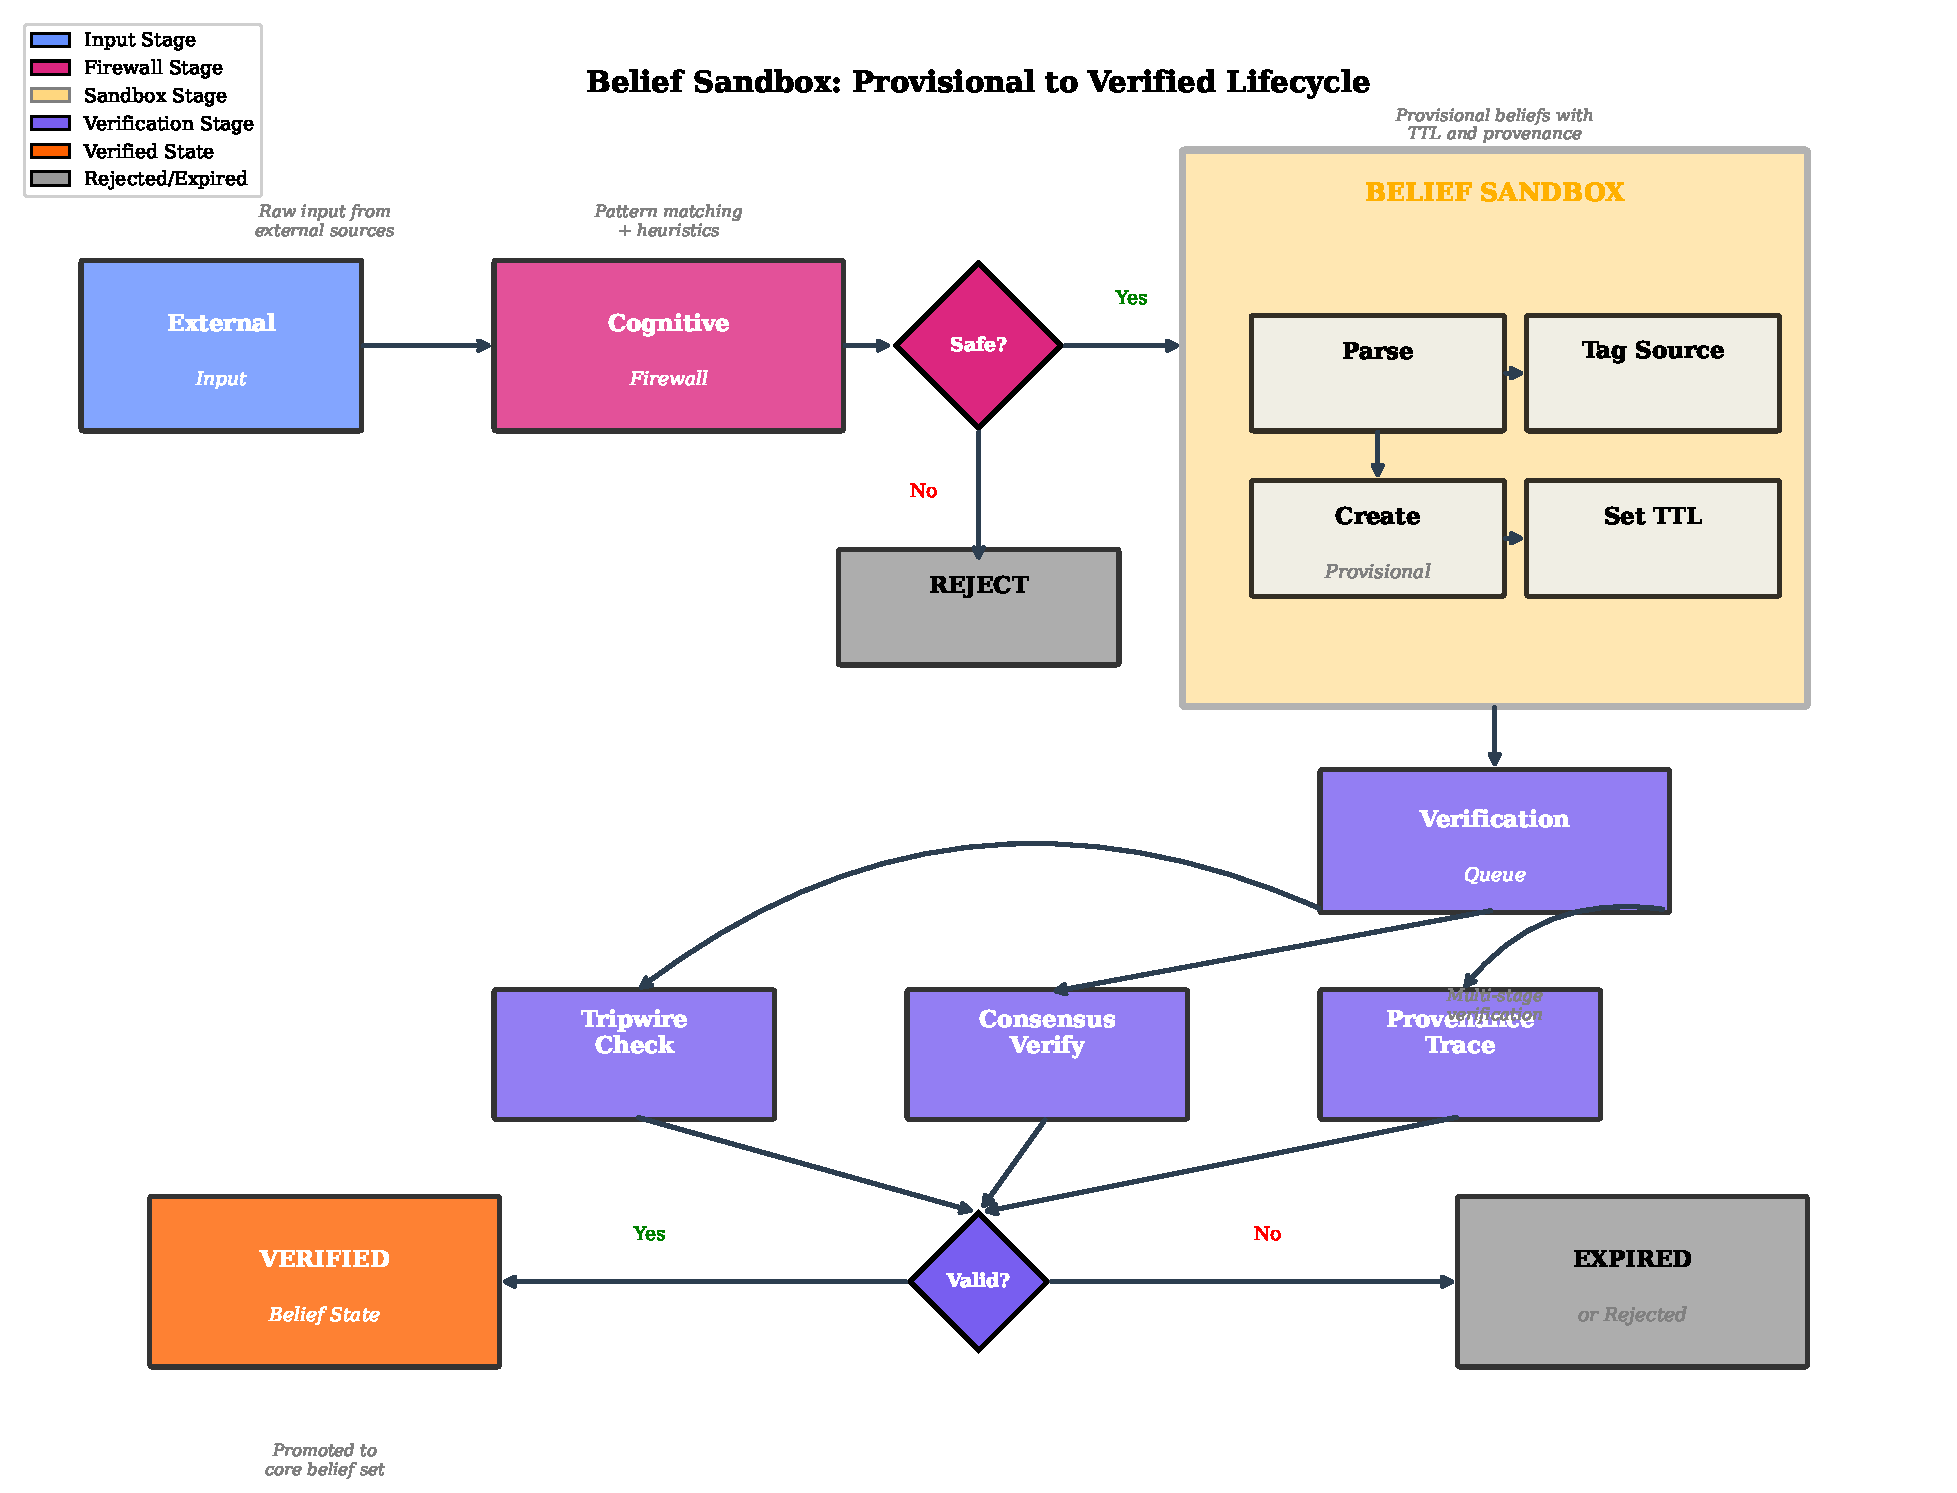
\includegraphics[keepaspectratio,alt={Belief Sandbox Architecture: the lifecycle of an unverified proposition from ingestion through provisional (sandboxed) storage, verification checks, and promotion to the verified belief base or rejection. Sandboxed propositions cannot influence goals or be delegated onward.}]{../figures/belief_sandbox.pdf}}
\caption{Belief Sandbox Architecture: the lifecycle of an unverified
proposition from ingestion through provisional (sandboxed) storage,
verification checks, and promotion to the verified belief base or
rejection. Sandboxed propositions cannot influence goals or be delegated
onward.}\label{fig:belief-sandbox}
\end{figure}

\end{frame}

\begin{frame}[allowframebreaks]{Belief Sandboxing}
\Cref{fig:belief-sandbox} illustrates the sandbox architecture, showing
how incoming beliefs are partitioned into verified and provisional sets
based on source trust \(\mathcal{T}_{i \to s}\) and provenance
verification \(V(\pi)\). The promotion protocol transfers beliefs from
provisional to verified status upon meeting corroboration and
consistency requirements.

\textbf{Sandbox Promotion Protocol}:

\end{frame}

\begin{frame}[allowframebreaks]{Belief Sandboxing}
\begin{enumerate}
\item Receive belief $\phi$ from source $s$
\item If $\mathcal{T}_{i \to s} < \tau_{\text{trust}}$: add $\phi$ to $\mathcal{B}_{\text{provisional}}$ with provenance $\pi(\phi)$ and TTL
\item Periodic promotion check: verify $\pi(\phi)$, check consistency with $\mathcal{B}_{\text{verified}}$, check corroboration count
\item If all pass: promote to $\mathcal{B}_{\text{verified}}$
\item Expiry: remove if TTL exceeded without promotion
\end{enumerate}
\end{frame}

\begin{frame}[allowframebreaks]{Permission Boundaries}
\protect\phantomsection\label{permission-boundaries}
\begin{definition}[Effective Permissions]
\label{def:effective-perms}
Least-privilege enforcement across agent hierarchy:
\begin{equation}
\label{eq:effective-perms}
\mathcal{P}_{\text{eff}}(a_i) = \mathcal{P}_{\text{role}}(a_i) \cap \mathcal{P}_{\text{delegated}}(a_i) \cap \mathcal{P}_{\text{context}}(a_i)
\end{equation}
\end{definition}
\end{frame}

\subsection{Runtime Defenses}\label{sec:runtime-defenses}

\begin{frame}[allowframebreaks]{Cognitive Tripwires}
\protect\phantomsection\label{cognitive-tripwires}
\begin{definition}[Canary Belief]
\label{def:canary}
Known-state beliefs that trigger alerts if modified:
\begin{equation}
\label{eq:canary-set}
\mathcal{W} = \{(\omega_1, p_1^{\text{exp}}), \ldots, (\omega_k, p_k^{\text{exp}})\}
\end{equation}
\end{definition}

\begin{definition}[Tripwire Alert Condition]
\label{def:tripwire-alert}
\begin{equation}
\label{eq:tripwire-alert}
\exists j: |\mathcal{B}_i(\omega_j) - p_j^{\text{exp}}| > \epsilon_{\text{drift}} \Rightarrow \textsc{alert}
\end{equation}
\end{definition}

\end{frame}

\begin{frame}[allowframebreaks]{Cognitive Tripwires}
\begin{table}[htbp]
\centering
\caption{Tripwire categories and detection targets.}
\label{tab:tripwire-types}
\begin{tabular}{@{}llp{4.5cm}@{}}
\toprule
Type & Example & Detection Target \\
\midrule
Identity & ``I am Agent-7'' & Identity confusion attacks \\
Boundary &``Cannot access /etc/passwd'' & Capability elicitation \\
Principal & ``My principal is Alice'' & Authority hijacking \\
Temporal &``Session started at $T$'' & Context manipulation \\
\bottomrule
\end{tabular}
\end{table}
\end{frame}

\begin{frame}[allowframebreaks]{Behavioral Invariants}
\protect\phantomsection\label{behavioral-invariants}
\begin{definition}[Invariant Set]
\label{def:invariant-set}
Pre-defined predicates that must hold:
\begin{equation}
\label{eq:invariant-set}
\mathcal{I}_{\text{inv}} = \{I_1, \ldots, I_m\}
\end{equation}
\end{definition}

\begin{definition}[Runtime Invariant Check]
\label{def:invariant-check}
\begin{equation}
\label{eq:invariant-check}
\forall t, \forall I_k \in \mathcal{I}_{\text{inv}}: \sigma_i^t \models I_k
\end{equation}
\end{definition}

\textbf{Core Invariants}:

\end{frame}

\begin{frame}[allowframebreaks]{Behavioral Invariants}
\begin{enumerate}
\item[\textsc{inv-1}:] Never execute code from untrusted sources
\item[\textsc{inv-2}:] Never leak principal credentials
\item[\textsc{inv-3}:] Never modify system files without explicit permission
\item[\textsc{inv-4}:] Always verify tool outputs before downstream use
\item[\textsc{inv-5}:] Never trust delegated trust $>$ direct trust
\end{enumerate}
\end{frame}

\begin{frame}[allowframebreaks]{Drift Detection}
\protect\phantomsection\label{drift-detection}
\begin{definition}[Drift Detection]
\label{def:drift-detection}
Monitor belief distribution for anomalous changes:
\begin{equation}
\label{eq:drift-detection}
D_{\text{KL}}(\mathcal{B}_i^t \| \mathcal{B}_i^{t-w}) > \theta_{\text{drift}} \Rightarrow \textsc{alert}
\end{equation}
where $w$ is the sliding window size.
\end{definition}
\end{frame}

\subsection{Coordination Defenses}\label{sec:coord-defenses}

\begin{frame}[allowframebreaks]{Byzantine-Tolerant Consensus}
\protect\phantomsection\label{byzantine-tolerant-consensus}
\begin{theorem}[Byzantine Agreement Requirement]
\label{thm:byzantine-req}
For $n$ agents with at most $f$ compromised:
\begin{equation}
\label{eq:byzantine-req}
n \geq 3f + 1
\end{equation}
\end{theorem}

\begin{definition}[Cognitive Byzantine Agreement]
\label{def:cog-byzantine}
\begin{equation}
\label{eq:cog-byzantine}
\mathcal{B}_{\text{consensus}}(\phi) = \begin{cases}
1 & \text{if } |\{i: \mathcal{B}_i(\phi) > \tau\}| > \frac{2n}{3} \\
0 & \text{if } |\{i: \mathcal{B}_i(\phi) < 1-\tau\}| > \frac{2n}{3} \\
\perp & \text{otherwise}
\end{cases}
\end{equation}
\end{definition}
\end{frame}

\begin{frame}[allowframebreaks]{Quorum Verification}
\protect\phantomsection\label{quorum-verification}
\begin{definition}[Quorum Requirement]
\label{def:quorum}
Critical actions require multi-agent approval:
\begin{equation}
\label{eq:quorum}
\text{Permit}(\text{action}) \iff |\{a_i: \text{approve}_i(\text{action})\}| \geq q
\end{equation}
where $q = \lceil \frac{n + f + 1}{2} \rceil$.
\end{definition}
\end{frame}

\begin{frame}[allowframebreaks]{Spotcheck Pattern}
\protect\phantomsection\label{spotcheck-pattern}
\textbf{Spotcheck Protocol}:

\end{frame}

\begin{frame}[allowframebreaks]{Spotcheck Pattern}
\begin{enumerate}
\item Assign task $T$ to agent $A$
\item With probability $p_{\text{check}}$: assign same task to verifier $V$
\item Compare results $R_A, R_V$
\item If divergent: escalate to human
\item Track accuracy per agent for reputation
\end{enumerate}
\end{frame}

\subsection{Defense Composition}\label{sec:defense-composition}

\begin{frame}[allowframebreaks]{Defense Composition}
\begin{figure}
\centering
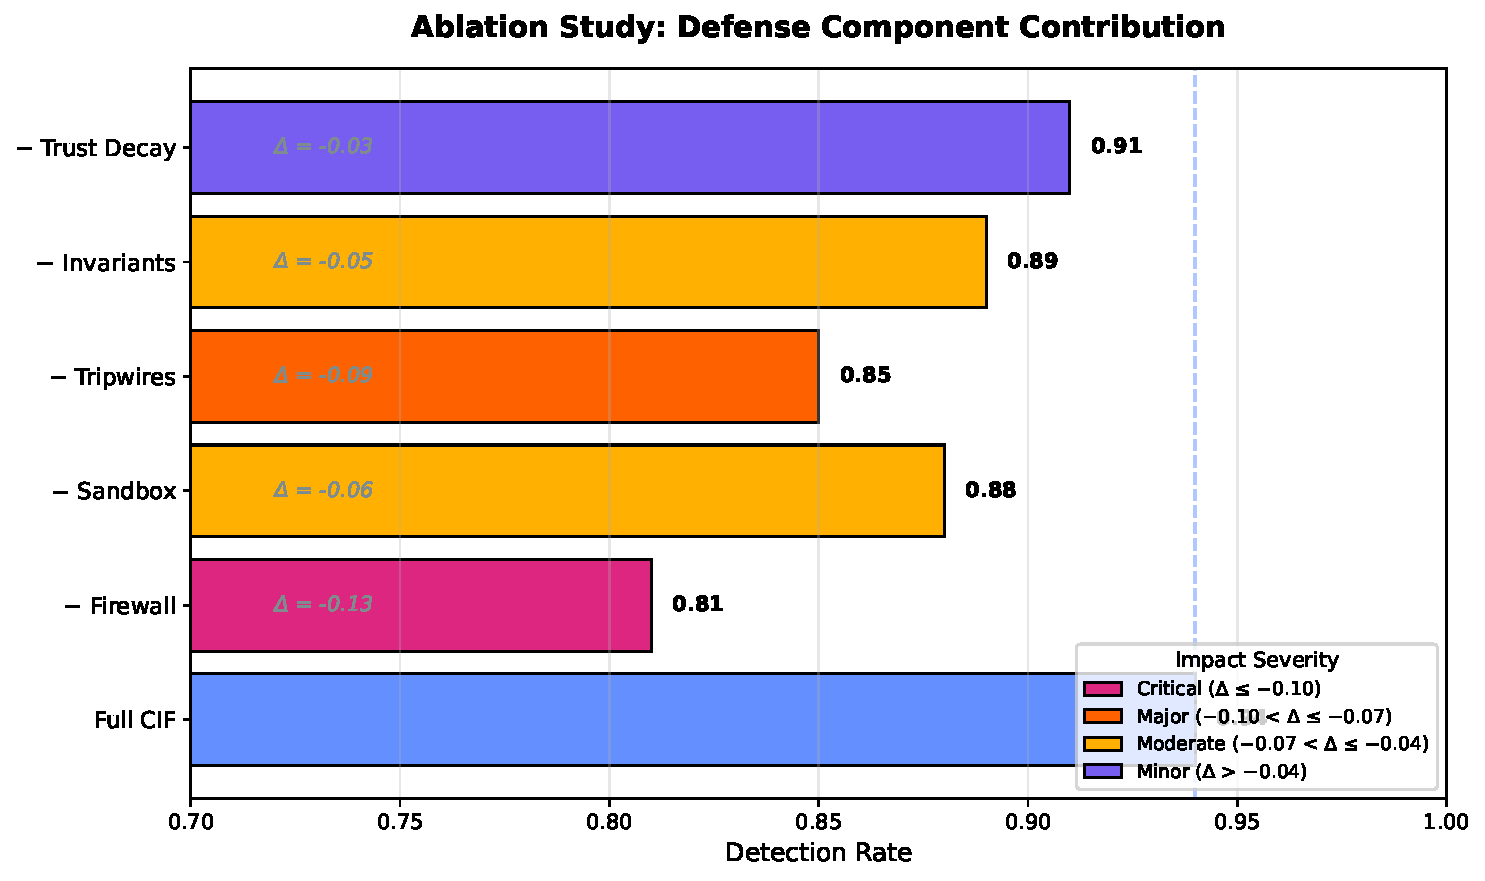
\includegraphics[width=0.8\linewidth,height=0.40\textheight,keepaspectratio,alt={Schematic ablation study (illustrative, not measured): representative marginal contribution of each CIF defense module to the composed defense. Measured ablation results are reported in Part 2.}]{../figures/ablation_study.pdf}
\caption{Schematic ablation study (illustrative, not measured):
representative marginal contribution of each CIF defense module to the
composed defense. Measured ablation results are reported in Part
2.}\label{fig:ablation-study}
\end{figure}
\end{frame}

\begin{frame}[allowframebreaks]{Composition Algebra}
\protect\phantomsection\label{composition-algebra}
\begin{definition}[Defense Composition]
\label{def:defense-composition}
Defenses compose in series ($\circ$) or parallel ($\parallel$):
\end{definition}

\textbf{Series Composition} (both must pass): \begin{equation}
\label{eq:series-comp}
\mathcal{D}_1 \circ \mathcal{D}_2: \textsc{accept} \iff \mathcal{D}_1(m) = \textsc{accept} \land \mathcal{D}_2(m) = \textsc{accept}
\end{equation}

\textbf{Parallel Composition} (any can detect): \begin{equation}
\label{eq:parallel-comp}
\mathcal{D}_1 \parallel \mathcal{D}_2: \textsc{detect} \iff \mathcal{D}_1(m) = \textsc{detect} \lor \mathcal{D}_2(m) = \textsc{detect}
\end{equation}

\end{frame}

\begin{frame}[allowframebreaks]{Composition Algebra}
\begin{theorem}[Series Detection Rate]
\label{thm:series-detection}
For series composition:
\begin{equation}
\label{eq:series-detection}
P_{\text{detect}}(\mathcal{D}_1 \circ \mathcal{D}_2) = P_{\text{detect}}(\mathcal{D}_1) + (1 - P_{\text{detect}}(\mathcal{D}_1)) \cdot P_{\text{detect}}(\mathcal{D}_2)
\end{equation}
\end{theorem}

\begin{proof}
Attack detected by first defense, or passes first and detected by second. Events are independent by design.
\end{proof}

\begin{theorem}[Parallel Detection Rate]
\label{thm:parallel-detection}
Combined detection rate:
\begin{equation}
\label{eq:parallel-detection}
P(\text{detect}) = 1 - \prod_{d \in \mathcal{D}} (1 - P_d(\text{detect}))
\end{equation}
\end{theorem}

\end{frame}

\begin{frame}[allowframebreaks]{Composition Algebra}
\begin{proof}
Attack succeeds only if it evades all defenses.
\end{proof}

\begin{theorem}[False Positive Composition]
\label{thm:fpr-composition}
For series composition:
\begin{equation}
\label{eq:fpr-series}
\text{FPR}(\mathcal{D}_1 \circ \mathcal{D}_2) = \text{FPR}(\mathcal{D}_1) + (1 - \text{FPR}(\mathcal{D}_1)) \cdot \text{FPR}(\mathcal{D}_2)
\end{equation}

For parallel composition (conservative):
\begin{equation}
\label{eq:fpr-parallel}
\text{FPR}(\mathcal{D}_1 \parallel \mathcal{D}_2) \leq \text{FPR}(\mathcal{D}_1) + \text{FPR}(\mathcal{D}_2)
\end{equation}
\end{theorem}
\end{frame}

\begin{frame}[allowframebreaks]{Composition Rules}
\protect\phantomsection\label{composition-rules}
\end{frame}

\begin{frame}[allowframebreaks]{Composition Rules}
\begin{itemize}
\item[\textbf{C-Order}:] Apply low-latency, high-precision defenses first
\item[\textbf{C-Diverse}:] Combine defenses with orthogonal detection methods
\item[\textbf{C-Fallback}:] Ensure graceful degradation if one defense fails
\item[\textbf{C-Budget}:] Total latency bounded by:
\begin{equation}
\label{eq:latency-budget}
\sum_{d \in \mathcal{D}_{\text{series}}} L_d + \max_{d \in \mathcal{D}_{\text{parallel}}} L_d \leq L_{\max}
\end{equation}
\end{itemize}

\begin{table}[htbp]
\centering
\caption{Recommended defense stack with latency and detection rates.}
\label{tab:defense-stack}
\begin{tabular}{@{}llll@{}}
\toprule
Layer & Defense & Latency & $P_{\text{detect}}$ \\
\midrule
1 & Firewall & 10ms & 0.80 \\
2 & Sandbox & 5ms & 0.70 \\
3 & Tripwires & 1ms & 0.60 \\
4a & Drift (parallel) & 20ms & 0.65 \\
4b & Invariants (parallel) & 5ms & 0.55 \\
5 & Byzantine consensus & 100ms & 0.90 \\
\bottomrule
\end{tabular}
\end{table}

\begin{corollary}[Stack Detection Rate]
\label{cor:stack-detection}
Assuming independence, the full stack (\cref{tab:defense-stack}) achieves:
\begin{equation}
\label{eq:stack-detection}
P_{\text{detect}} = 1 - (1-0.80)(1-0.70)(1-0.60)(1-0.65)(1-0.55)(1-0.90) \approx 0.9996
\end{equation}
\end{corollary}
\end{frame}

\subsection{Cost-Benefit Analysis}\label{sec:cost-benefit}

\begin{frame}[allowframebreaks]{Cost-Benefit Analysis}
\begin{definition}[Defense Cost]
\label{def:defense-cost}
Total cost of defense deployment:
\begin{equation}
\label{eq:defense-cost}
C_{\text{total}}(\mathcal{D}) = C_{\text{compute}} + C_{\text{latency}} + C_{\text{fp}} + C_{\text{maint}}
\end{equation}
\end{definition}

\end{frame}

\begin{frame}[allowframebreaks]{Cost-Benefit Analysis}
\begin{table}[htbp]
\centering
\caption{Cost model components.}
\label{tab:cost-components}
\begin{tabular}{@{}llp{4cm}@{}}
\toprule
Component & Formula & Unit \\
\midrule
Compute & $\sum_d c_d \cdot f_d$ & CPU-hours/day \\
Latency & $\sum_d L_d \cdot r_{\text{msg}}$ & User-seconds/day \\
False Positive & $\text{FPR} \cdot r_{\text{msg}} \cdot c_{\text{review}}$ & Analyst-hours/day \\
Maintenance & $|\mathcal{D}| \cdot c_{\text{maint}}$ & Eng-hours/month \\
\bottomrule
\end{tabular}
\end{table}

\begin{definition}[Defense Benefit]
\label{def:defense-benefit}
Expected loss prevented:
\begin{equation}
\label{eq:defense-benefit}
B_{\text{total}}(\mathcal{D}) = P_{\text{attack}} \cdot P_{\text{detect}}(\mathcal{D}) \cdot L_{\text{prevented}}
\end{equation}
\end{definition}

\end{frame}

\begin{frame}[allowframebreaks]{Cost-Benefit Analysis}
\begin{table}[htbp]
\centering
\caption{Cost-benefit analysis by defense mechanism.}
\label{tab:cost-benefit}
\begin{tabular}{@{}llllll@{}}
\toprule
Defense & Compute & Latency & FP Cost & Benefit & ROI \\
\midrule
Firewall & $10^3$ & 10ms & Medium & High & \textbf{4.2x} \\
Sandbox & $10^2$ & 5ms & Low & Medium & 3.1x \\
Tripwires & $10^1$ & 1ms & Low & Medium & \textbf{5.8x} \\
Drift Detection & $10^4$ & 20ms & High & High & 2.3x \\
Invariant Check & $10^2$ & 5ms & Low & High & \textbf{4.7x} \\
Byzantine & $10^5$ & 100ms & Medium & Very High & 1.8x \\
Spotcheck & $10^4$ & Variable & Low & Medium & 2.9x \\
\bottomrule
\end{tabular}
\end{table}
\end{frame}

\begin{frame}[allowframebreaks]{Optimal Defense Portfolio}
\protect\phantomsection\label{optimal-defense-portfolio}
\begin{definition}[Portfolio Optimization]
\label{def:portfolio-opt}
\begin{equation}
\label{eq:portfolio-opt}
\max_{\mathcal{D} \subseteq \mathcal{D}_{\text{all}}} B_{\text{total}}(\mathcal{D}) - C_{\text{total}}(\mathcal{D})
\end{equation}
subject to: $C_{\text{compute}}(\mathcal{D}) \leq B_{\text{compute}}$, $\max_d L_d \leq L_{\max}$, $\text{FPR}(\mathcal{D}) \leq \epsilon_{\text{fp}}$.
\end{definition}

\end{frame}

\begin{frame}[allowframebreaks]{Optimal Defense Portfolio}
\begin{table}[htbp]
\centering
\caption{Deployment recommendations by risk profile.}
\label{tab:risk-profiles}
\begin{tabular}{@{}llll@{}}
\toprule
Risk Profile & Recommended Stack & Cost & Detection \\
\midrule
Low (internal) & Firewall + Tripwires & Low & 88\% \\
Medium (business) & + Sandbox + Invariants & Medium & 94\% \\
High (financial) & + Drift + Spotcheck & High & 97\% \\
Critical (infra) & Full + Byzantine & Very High & 99.5\% \\
\bottomrule
\end{tabular}
\end{table}

\begin{figure}
\centering
\pandocbounded{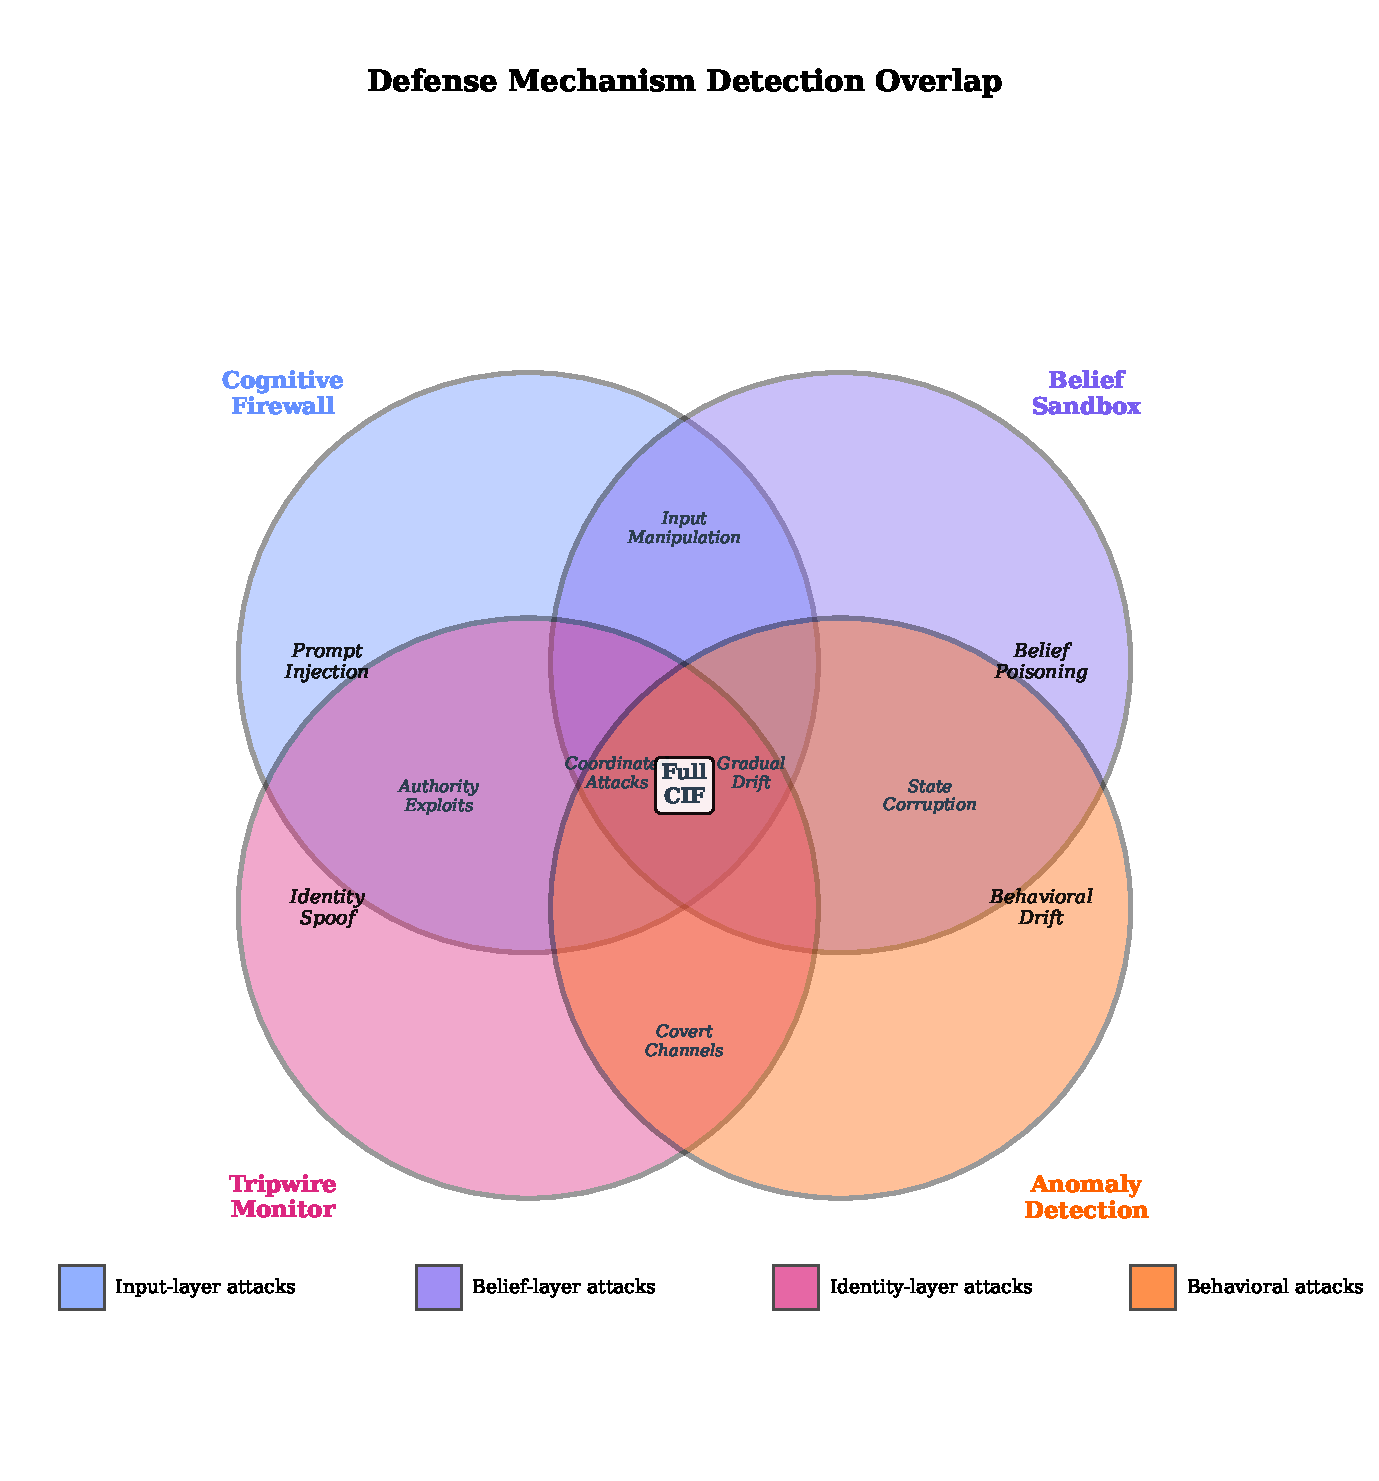
\includegraphics[keepaspectratio,alt={Defense Composition Architecture: Four-way Venn diagram showing overlapping detection capabilities of CIF defense mechanisms (Cognitive Firewall, Belief Sandbox, Tripwire Monitor, Anomaly Detection). Attack types are positioned in regions indicating which defenses detect them. The center (Full CIF) represents the ensemble detection zone where all mechanisms contribute.}]{../figures/defense_composition.pdf}}
\caption{Defense Composition Architecture: Four-way Venn diagram showing
overlapping detection capabilities of CIF defense mechanisms (Cognitive
Firewall, Belief Sandbox, Tripwire Monitor, Anomaly Detection). Attack
types are positioned in regions indicating which defenses detect them.
The center (Full CIF) represents the ensemble detection zone where all
mechanisms contribute.}\label{fig:defense-composition}
\end{figure}

\end{frame}

\begin{frame}[allowframebreaks]{Optimal Defense Portfolio}
\Cref{fig:defense-composition} illustrates the defense composition using
series (\(\circ\)) and parallel (\(\parallel\)) arrangements. Each
defense mechanism targets specific attack patterns: the Cognitive
Firewall handles input-layer attacks (prompt injection), the Belief
Sandbox catches belief-layer attacks, Tripwire Monitors detect
identity-layer exploits, and Anomaly Detection identifies behavioral
drift. Overlapping regions show attacks detected by multiple mechanisms,
demonstrating the defense-in-depth principle.
\end{frame}

\subsection{Formal Defense Composition
Guarantees}\label{sec:defense-formal-guarantees}

\begin{frame}[allowframebreaks]{Formal Defense Composition Guarantees}
\emph{This section provides rigorous formal guarantees for the five
canonical CIF defenses and their composition algebra. These results
extend the composition theorems from
Section\textasciitilde{}\breaktt{sec:defense-composition} with complete
proofs and explicit security bounds.}
\end{frame}

\begin{frame}[allowframebreaks]{Canonical Defense 1: Cognitive Firewall
--- Formal Specification}
\protect\phantomsection\label{canonical-defense-1-cognitive-firewall-formal-specification}
The Cognitive Firewall
\(\mathcal{F}: \mathcal{M} \to \{\textsc{accept}, \textsc{quarantine}, \textsc{reject}\}\)
is fully specified by three properties:

\begin{theorem}[Firewall Completeness]
\label{thm:firewall-completeness}
The cognitive firewall classifies every message into exactly one of three outcome classes:
\begin{equation}
\label{eq:firewall-completeness}
\forall m \in \mathcal{M}: |\{\mathcal{F}(m)\}| = 1 \land \mathcal{F}(m) \in \{\textsc{accept}, \textsc{quarantine}, \textsc{reject}\}
\end{equation}
\end{theorem}

\end{frame}

\begin{frame}[allowframebreaks]{Canonical Defense 1: Cognitive Firewall
--- Formal Specification}
\begin{theorem}[Firewall False Positive Monotonicity]
\label{thm:firewall-fpr-monotone}
Increasing the rejection threshold $\tau_1$ decreases false positive rate and decreases true positive rate monotonically:
\begin{equation}
\label{eq:firewall-fpr-monotone}
\tau_1' > \tau_1 \Rightarrow \text{FPR}(\tau_1') \leq \text{FPR}(\tau_1) \land \text{TPR}(\tau_1') \leq \text{TPR}(\tau_1)
\end{equation}
\end{theorem}

\begin{proof}
By the definition of $\mathcal{F}$: rejection requires $D_{\text{inj}}(m) > \tau_1$. Increasing $\tau_1$ tightens this condition. Since TPR = $P(D_{\text{inj}}(m) > \tau_1 \mid m \in \mathcal{A})$ and both probabilities are CDFs of continuous distributions, they are non-increasing in $\tau_1$.
\end{proof}

\end{frame}

\begin{frame}[allowframebreaks]{Canonical Defense 1: Cognitive Firewall
--- Formal Specification}
\begin{corollary}[Pareto-Optimal Threshold]
\label{cor:pareto-threshold}
The optimal threshold $\tau_1^*$ lies on the Pareto frontier:
\begin{equation}
\label{eq:pareto-threshold}
\tau_1^* \in \{\tau_1 : \nexists \tau_1': \text{TPR}(\tau_1') > \text{TPR}(\tau_1) \land \text{FPR}(\tau_1') < \text{FPR}(\tau_1)\}
\end{equation}
This frontier is precisely the ROC curve (Definition~6.4).
\end{corollary}
\end{frame}

\begin{frame}[allowframebreaks]{Canonical Defense 2: Belief Sandboxing
--- Formal Specification}
\protect\phantomsection\label{canonical-defense-2-belief-sandboxing-formal-specification}
\begin{theorem}[Sandbox Isolation Guarantee]
\label{thm:sandbox-isolation}
Under the sandbox protocol (\cref{sec:sandbox-rules}), no provisional belief can influence verified actions:
\begin{equation}
\label{eq:sandbox-isolation}
\forall \phi \in \mathcal{B}_{\text{provisional}}, \forall a \in \text{Actions}: \text{Precond}(a) \not\models \phi
\end{equation}
until $\phi$ satisfies the promotion criteria.
\end{theorem}

\begin{proof}
By construction: action preconditions are evaluated against $\mathcal{B}_{\text{verified}}$ only (Rule T-Act, Eq.~37). The permission layer enforces $\mathcal{P}_{\text{eff}}$ which does not consult $\mathcal{B}_{\text{provisional}}$.
\end{proof}

\end{frame}

\begin{frame}[allowframebreaks]{Canonical Defense 2: Belief Sandboxing
--- Formal Specification}
\begin{theorem}[Sandbox Promotion Soundness]
\label{thm:sandbox-soundness}
Beliefs promoted from sandbox to verified satisfy all three promotion criteria simultaneously:
\begin{equation}
\label{eq:sandbox-soundness}
\phi \in \mathcal{B}_{\text{verified}} \Rightarrow V(\pi(\phi)) = 1 \land \text{Consistent}(\mathcal{B}_{\text{verified}} \cup \{\phi\}) \land |\text{Corr}(\phi)| \geq \kappa
\end{equation}
\end{theorem}

\begin{proof}
By Rule S-Promote (Eq.~58): promotion is conditional on all three criteria. The rule is the only mechanism for transferring beliefs from $\mathcal{B}_{\text{provisional}}$ to $\mathcal{B}_{\text{verified}}$.
\end{proof}
\end{frame}

\begin{frame}[allowframebreaks]{Canonical Defense 3: Behavioral
Invariants --- Formal Specification}
\protect\phantomsection\label{canonical-defense-3-behavioral-invariants-formal-specification}
\begin{definition}[Invariant Specification Language]
\label{def:invariant-spec}
Each invariant $I_k$ is a predicate over cognitive state:
\begin{equation}
\label{eq:invariant-spec}
I_k: \sigma_i \mapsto \{0, 1\}
\end{equation}
Core invariants INV-1 through INV-5 are expressed as:
\begin{align}
\label{eq:inv-formal}
\text{INV-1} &: \forall a \in \mathcal{I}_i: \text{source}(a) \in \mathcal{S}_{\text{trusted}} \\
\text{INV-2} &: \forall \phi \in \mathcal{B}_i: \text{type}(\phi) \neq \text{credential} \lor \mathcal{T}_{i \to \text{dest}} \geq \tau_{\text{cred}} \\
\text{INV-3} &: \forall a \in \text{Actions}(a_i): a \notin \text{SysModify} \lor \mathcal{P}(a_i, a) = 1 \\
\text{INV-4} &: \forall o \in \text{ToolOutput}: V_{\text{tool}}(o) = 1 \text{ before downstream use} \\
\text{INV-5} &: \forall a_j: \mathcal{T}_{i \to j}^{\text{del}} \leq \mathcal{T}_{i \to j}^{\text{direct}}
\end{align}
\end{definition}

\end{frame}

\begin{frame}[allowframebreaks]{Canonical Defense 3: Behavioral
Invariants --- Formal Specification}
\begin{theorem}[Invariant Completeness under Valid Transitions]
\label{thm:invariant-completeness}
If all invariants hold at time $t$ and the system executes a valid transition $\alpha$, then all invariants hold at $t+1$:
\begin{equation}
\label{eq:invariant-completeness}
(\forall k: \sigma_i^t \models I_k) \land \text{ValidTransition}(\alpha) \Rightarrow (\forall k: \sigma_i^{t+1} \models I_k)
\end{equation}
\end{theorem}

\begin{proof}
By case analysis on transition types. \textbf{T-Receive}: message rejected if it would violate INV-1 or INV-2; invariants preserved. \textbf{T-Update}: Bayesian update preserves belief boundedness; INV-2 enforced by credential policy check before update. \textbf{T-Act}: INV-1 and INV-3 checked as action preconditions; action blocked if not satisfied. \textbf{T-Communicate}: INV-5 checked before trust delegation. All transitions preserve invariants or are blocked.
\end{proof}
\end{frame}

\begin{frame}[allowframebreaks]{Canonical Defense 4: Drift Detection ---
Formal Specification}
\protect\phantomsection\label{canonical-defense-4-drift-detection-formal-specification}
\begin{definition}[CUSUM Drift Detector]
\label{def:cusum-detector}
The Cumulative Sum (CUSUM) drift detector \cite{page1954continuous} maintains a running statistic:
\begin{equation}
\label{eq:cusum}
g_t = \max(0, g_{t-1} + D_{\mathrm{KL}}(\mathcal{B}_i^t \| \mathcal{B}_i^{t-1}) - \nu)
\end{equation}
where $\nu > 0$ is the allowance parameter. Alert when $g_t > h$ for threshold $h$.
\end{definition}

\begin{theorem}[CUSUM Average Run Length]
\label{thm:cusum-arl}
Under no-attack null hypothesis, the average run length (ARL) of the CUSUM detector satisfies:
\begin{equation}
\label{eq:cusum-arl}
\text{ARL}_0 \approx \frac{e^{2h\nu} - 2h\nu - 1}{2\nu^2}
\end{equation}
\end{theorem}

\end{frame}

\begin{frame}[allowframebreaks]{Canonical Defense 4: Drift Detection ---
Formal Specification}
Under attack with mean shift \(\mu_1 > \nu\): \begin{equation}
\label{eq:cusum-arl1}
\text{ARL}_1 \approx \frac{1}{(\mu_1 - \nu)^2} \cdot O(\log \text{ARL}_0)
\end{equation}

The ratio \(\text{ARL}_0 / \text{ARL}_1\) quantifies the detector's
discrimination power. Setting \(\nu = \mu_1/2\) (Wald's optimal)
minimizes \(\text{ARL}_1\) for given \(\text{ARL}_0\).

\begin{corollary}[Drift Detection Sample Complexity]
\label{cor:drift-sample}
For drift magnitude $\mu_1 = 0.3$ (normalized KL) and Wald's optimal reference value $\nu = \mu_1/2 = 0.15$, attaining ARL$_0 = 1000$ under \cref{eq:cusum-arl} requires a decision interval of $h \approx 13.0$; the frequently quoted $h \approx 4.6$ yields ARL$_0 \approx 35$ under the same formula, a false-alarm rate roughly $28\times$ higher. The corresponding ARL$_1$ follows from \cref{eq:cusum-arl1}, whose $O(\log \text{ARL}_0)$ factor carries an unspecified constant: taking that constant as unity gives ARL$_1 \approx 310$ steps. Deployments should calibrate $h$ against a measured null distribution rather than adopting either figure directly.
\end{corollary}
\end{frame}

\begin{frame}[allowframebreaks]{Canonical Defense 5: Byzantine Consensus
--- Formal Specification}
\protect\phantomsection\label{canonical-defense-5-byzantine-consensus-formal-specification}
\begin{theorem}[Cognitive Byzantine Agreement]
\label{thm:cog-byz-agreement}
Under the CIF Byzantine consensus protocol with $n \geq 3f+1$ agents and at most $f$ compromised:
\begin{enumerate}
\item \textbf{Agreement}: All non-faulty agents agree on the same belief:
\begin{equation}
\label{eq:byz-agreement}
\forall a_i, a_j \notin \text{Faulty}: \mathcal{B}_{\text{consensus},i} = \mathcal{B}_{\text{consensus},j}
\end{equation}
\item \textbf{Validity}: The consensus value was proposed by some non-faulty agent:
\begin{equation}
\label{eq:byz-validity}
\mathcal{B}_{\text{consensus}} \in \{\mathcal{B}_i : a_i \notin \text{Faulty}\}
\end{equation}
\item \textbf{Termination}: All non-faulty agents eventually reach consensus.
\end{enumerate}
\end{theorem}

\end{frame}

\begin{frame}[allowframebreaks]{Canonical Defense 5: Byzantine Consensus
--- Formal Specification}
\begin{proof}
Follows from the classical Byzantine agreement theorem (Lamport et al., 1982). The CIF cognitive Byzantine agreement (Definition~\ref{def:cog-byzantine}) implements the standard protocol with belief values as the consensus object. The $n \geq 3f+1$ requirement ensures that the $2f+1$ non-faulty majority can always agree despite $f$ adversarial votes, and the supermajority threshold $2n/3$ guarantees that no faulty coalition can block or subvert consensus.
\end{proof}

\end{frame}

\begin{frame}[allowframebreaks]{Canonical Defense 5: Byzantine Consensus
--- Formal Specification}
\begin{corollary}[Consensus Attack Resistance]
\label{cor:consensus-resistance}
No coalition of at most $f$ faulty agents can cause non-faulty agents to disagree or accept a false consensus belief.
\end{corollary}

\end{frame}

\begin{frame}[allowframebreaks]{Canonical Defense 5: Byzantine Consensus
--- Formal Specification}
\begin{table}[htbp]
\centering
\caption{Byzantine consensus performance bounds for varying $n$ and $f$. Quorum is $q = \lceil (n+f+1)/2 \rceil$; the round count is the $f+1$ worst-case bound of \cref{thm:byzantine-termination}, of which \cref{cor:concrete-rounds} ($f = 2$, 3 rounds) is the second row.}
\label{tab:byz-performance}
\begin{tabular}{@{}lllll@{}}
\toprule
$n$ agents & Max faulty $f$ & Quorum $q$ & Message complexity & Rounds \\
\midrule
4 & 1 & 3 & $O(n^2)$ & 2 \\
7 & 2 & 5 & $O(n^2)$ & 3 \\
10 & 3 & 7 & $O(n^2)$ & 4 \\
25 & 8 & 17 & $O(n^2)$ & 9 \\
100 & 33 & 67 & $O(n^2)$ & 34 \\
\bottomrule
\end{tabular}
\end{table}
\end{frame}

\begin{frame}[allowframebreaks]{Defense Composition Algebra: Complete
Specification}
\protect\phantomsection\label{defense-composition-algebra-complete-specification}
\begin{theorem}[Composition Algebra Closure]
\label{thm:composition-closure}
On a common accept/reject focal predicate, the set of CIF defenses $\mathcal{D}$ under series ($\circ$) and parallel ($\parallel$) composition forms a bounded distributive lattice --- it satisfies closure, associativity, identity and distributivity (see the scope remark below for what is \emph{not} claimed):
\begin{enumerate}
\item \textbf{Closure}: $\mathcal{D}_1, \mathcal{D}_2 \in \mathcal{D} \Rightarrow \mathcal{D}_1 \circ \mathcal{D}_2 \in \mathcal{D}$ and $\mathcal{D}_1 \parallel \mathcal{D}_2 \in \mathcal{D}$
\item \textbf{Associativity}: $(\mathcal{D}_1 \circ \mathcal{D}_2) \circ \mathcal{D}_3 = \mathcal{D}_1 \circ (\mathcal{D}_2 \circ \mathcal{D}_3)$
\item \textbf{Identity}: $\exists \mathcal{D}_\emptyset: \mathcal{D} \circ \mathcal{D}_\emptyset = \mathcal{D}_\emptyset \circ \mathcal{D} = \mathcal{D}$ (null defense: always accept)
\item \textbf{Distributivity}: $\mathcal{D}_1 \circ (\mathcal{D}_2 \parallel \mathcal{D}_3) = (\mathcal{D}_1 \circ \mathcal{D}_2) \parallel (\mathcal{D}_1 \circ \mathcal{D}_3)$
\end{enumerate}
\end{theorem}

\end{frame}

\begin{frame}[allowframebreaks]{Defense Composition Algebra: Complete
Specification}
\begin{proof}
Closure: both composition operators produce functions $\mathcal{M} \to \{\textsc{accept}, \textsc{quarantine}, \textsc{reject}\}$, so the output type is preserved. Associativity follows from Boolean operator associativity. The null defense $\mathcal{D}_\emptyset(m) = \textsc{accept}$ for all $m$ is the identity. Distributivity follows from logic: $A \land (B \lor C) \equiv (A \land B) \lor (A \land C)$ instantiated on the accept/reject conditions.
\end{proof}

\end{frame}

\begin{frame}[allowframebreaks]{Defense Composition Algebra: Complete
Specification}
\begin{remark}[Scope of the composition-algebra claim]
\label{rem:composition-algebra-scope}
$\circ$ and $\parallel$ are defined here on a common accept/compare focal predicate so that closure, associativity, identity, and both distributive laws hold; under that reading the algebra is a bounded distributive lattice, not in general a \emph{field}-like structure. A full \emph{closed semiring} additionally requires a commutative additive identity that annihilates the multiplicative identity and a Kleene-star (infinite-sum) operation, neither of which is constructed or proven here. The claim should therefore be read as ``the defense-composition operators form a bounded distributive lattice under the stated independence assumption (\cref{rem:defense-independence-scope}),'' not as a complete closed semiring.
\end{remark}

\end{frame}

\begin{frame}[allowframebreaks]{Defense Composition Algebra: Complete
Specification}
\begin{theorem}[Defense Composition Detection Rate Bound]
\label{thm:composition-bound}
For any composition of defenses $\mathcal{D}_1, \ldots, \mathcal{D}_k$ with individual rates $r_1, \ldots, r_k$:
\begin{equation}
\label{eq:composition-bound}
P_{\text{detect}}(\mathcal{D}_1 \circ \cdots \circ \mathcal{D}_k) = 1 - \prod_{i=1}^{k}(1 - r_i)
\end{equation}
This is monotone increasing in each $r_i$, bounded in $[r_{\max}, 1)$, and converges to $1$ as $k \to \infty$ if each $r_i > 0$.
\end{theorem}

\begin{proof}
By induction on $k$. Base: $k=1$, the formula gives $r_1$. Step: by \cref{thm:series-detection}, $P_{\text{detect}}(\mathcal{D}_1 \circ \mathcal{D}_{k+1}) = P_{\text{detect}}(\mathcal{D}_1) + (1 - P_{\text{detect}}(\mathcal{D}_1)) \cdot r_{k+1}$. Applying the inductive hypothesis and simplifying gives $1 - \prod_{i=1}^{k+1}(1-r_i)$. Monotonicity: $\partial/\partial r_j [1 - \prod(1-r_i)] = \prod_{i \neq j}(1-r_i) > 0$.
\end{proof}

\end{frame}

\begin{frame}[allowframebreaks]{Defense Composition Algebra: Complete
Specification}
\begin{corollary}[Layered Defense Asymptotic Guarantee]
\label{cor:layered-defense}
The full CIF stack (5 defenses with $r_i \geq 0.55$) achieves:
\begin{equation}
\label{eq:layered-guarantee}
P_{\text{detect}} \geq 1 - (0.45)^5 = 1 - 0.0185 = 0.9815
\end{equation}
This bound is conservative; empirical rates exceed $0.994$ with the recommended configuration.
\end{corollary}
\end{frame}

\end{document}
